\documentclass[10pt,twocolumn]{article}
\usepackage[margin=0.72in]{geometry}
\usepackage{fontspec}
\usepackage{amsmath,amssymb}
\usepackage{graphicx}
\usepackage{booktabs}
\usepackage{microtype}
\usepackage[hidelinks]{hyperref}
\hypersetup{
  unicode=true,
  pdftitle={Beyond Contraction: Contextual Evidence Separates Lexical Senses Without Universal Within-Sense Collapse},
  pdfauthor={Hồ Ngọc Huy},
  pdfsubject={Exploratory preprint on contextual lexical representation geometry and lexical ambiguity},
  pdfkeywords={contextual embeddings, lexical ambiguity, word sense disambiguation, representation geometry, linear probing, LEACE}
}
\usepackage{xcolor}
\usepackage{enumitem}
\setlist{nosep,leftmargin=*}
\setlength{\columnsep}{0.22in}
\setlength{\parindent}{1em}
\setlength{\parskip}{0pt}
\title{\vspace{-1.5em}\textbf{Beyond Contraction: Contextual Evidence Separates Lexical Senses Without Universal Within-Sense Collapse}}
\author{Hồ Ngọc Huy\\\small Undergraduate, University of Science, VNU-HCM\\\small ORCID: \href{https://orcid.org/0009-0007-4156-352X}{0009-0007-4156-352X}}
\date{August 2026}

\begin{document}
\maketitle
\vspace{-1em}

\begin{abstract}
Context can make the intended sense of an ambiguous word easier to recover. A tempting geometric interpretation is that representations should therefore collapse into a tighter same-sense cluster. We test that interpretation directly in frozen BERT-base, RoBERTa-base, and DeBERTa-v3-base representations of 19 coarse ambiguous English nouns. When sense-diagnostic context is compared with the same amount of randomly selected context, between-sense separation increases in every aggregate model--layer--evidence cell, while within-sense dispersion can decrease, remain nearly unchanged, or increase. A nested intervention then holds the existing context fixed and adds one diagnostic or matched control cue. Diagnostic cues increase linear sense accessibility and produce updates that align more with a supervised sense-discriminative subspace, but they also change broader representational structure. A newly fit decoder recovers a fixed low-dimensional summary of the previous context about as well as controls, whereas a decoder trained on the pre-cue state transfers less well. Label-independent local context, LEACE erasure, and RAW-C provide complementary checks. The narrow conclusion is that lexical disambiguation need not be geometric contraction. We use \emph{sense-directed reorganization} only as a descriptive name for the observed pattern, not as a universal computational mechanism.
\end{abstract}

\section{A simple geometric question}
A word such as \emph{bank} can denote a financial institution or a river edge. After seeing \emph{mortgage}, the financial sense becomes much easier to identify. It is natural to picture this as a shrinking region of possible meanings,
\begin{equation}
R_0 \supset R_1 \supset R_2 \supset \cdots .
\end{equation}
That picture mixes two objects. A contextual encoder produces one vector $h=E(w,c)$ for one occurrence. A ``cloud'' appears only after collecting vectors from many contexts. Its spread is therefore not itself a posterior distribution over lexical senses. Two sentences can make the same sense unambiguous while differing in event, topic, participants, syntax, or discourse role.

The paper tests the corresponding geometric inference rather than semantic uncertainty itself:
\begin{equation}
\text{sense accessibility}\neq\text{within-sense dispersion}.
\end{equation}

Recent work shows strong layer- and architecture-dependent sense differentiation \cite{ma2025,riviere2025}, structured context-induced transformations \cite{hu2026,xiong2026}, and cases where embedding similarity diverges from functional sense distinctions \cite{scott2026}. Mechanistic work also identifies attention components that contribute to disambiguation \cite{rivieretrott2025}. Our axis is complementary: rather than varying network depth alone, we manipulate how much \emph{sense-relevant contextual evidence} is available.

\paragraph{Scope before results.}
We do not estimate $H(S\mid C)$, equate probe performance with model understanding, treat a supervised subspace as an independently discovered privileged axis, or claim that a low-dimensional reconstruction target captures all context. The oracle cue selection below is a measurement intervention, not a deployable WSD method. These restrictions prevent a geometric observation from silently becoming a stronger semantic or mechanistic claim.

\section{Experimental design}
\subsection{Data and representations}
We use CoarseWSD-20 \cite{loureiro2021}. After within-word balancing and context-availability filtering, 19 lexical items remain; \emph{deck} falls below the held-out minimum. The statistical unit is the lexical item, not individual token pairs.

We freeze BERT-base-uncased, RoBERTa-base, and DeBERTa-v3-base and extract target-token representations from layers 4, 8, and 12, averaging target subwords when needed. Because model families differ in scale and anisotropy \cite{ethayarajh2019,timkey2021}, cross-architecture conclusions rely on signs and within-model trajectories rather than raw magnitude comparisons.

For sense $s$ with probability $p_s$, sense mean $\mu_s$, and global mean $\mu$, we decompose total covariance trace into
\begin{align}
W&=\sum_s p_s\,\mathrm{tr}\,\mathrm{Cov}(Z\mid S=s),\\
B&=\sum_s p_s\lVert\mu_s-\mu\rVert_2^2,
\end{align}
so that $\mathrm{tr}\,\mathrm{Cov}(Z)=W+B$. Here $W$ measures within-sense dispersion and $B$ measures between-sense centroid separation.

Linear sense accessibility is the held-out reduction in negative log likelihood relative to a null predictor,
\begin{equation}
I_V(S;Z)=\mathrm{NLL}_{\mathrm{null}}-\mathrm{NLL}_{\mathrm{probe}},
\end{equation}
reported in nats for a fixed linear probe family. This is deliberately called \emph{linear accessibility}, not mutual information \cite{hewitt2019}.

\subsection{Experiment A: controlled evidence}
Token--sense PMI is estimated from the official training split only. For each held-out occurrence, an oracle ordering reveals remaining context tokens with highest PMI for the gold sense. Five random reveal orderings provide matched context-quantity controls. We compare $k\in\{1,2,4,8,16\}$ visible tokens. BERT additionally receives a deletion-based artifact check.

The test is simple: if disambiguation generally behaves like contraction, diagnostic context should not only improve sense differentiation; it should also reliably reduce $W$ relative to equally large random context.

\subsection{Experiment B: one cue from the same state}
Each occurrence starts from the same label-independent random base context of $m\in\{2,4,8\}$ tokens. We then add either the highest-PMI remaining diagnostic cue or a matched control cue:
\begin{align}
h_{\text{base}}&=E(w,C_{\text{base}}),\\
h_{\text{diag}}&=E(w,C_{\text{base}}\cup\{c_{\text{diag}}\}),\\
h_{\text{ctrl}}&=E(w,C_{\text{base}}\cup\{c_{\text{ctrl}}\}).
\end{align}
We ask four separate questions: does sense become more linearly accessible; does the update $\delta=h_{\text{post}}-h_{\text{pre}}$ place more energy in a supervised sense-discriminative subspace; does broader structure remain similar to the base state (CKA/RSA); and does a fixed lexical summary of the old context remain recoverable?

The sense subspace is the span of training-set sense-mean offsets $\{\mu_s-\mu\}$. Because the probe and this subspace share gold labels, their association is descriptive evidence of sense-structured change, not an unsupervised discovery.

For old-context reconstruction, the pre-cue context is encoded with a training-only TF-IDF unigram/bigram vectorizer, reduced with TruncatedSVD to at most 64 dimensions, and row-normalized. Ridge decoders predict that target from the token representation. We compare a decoder fit separately after each condition with transfer of a decoder trained on the base state without refitting. The target is a lexical summary, not a complete representation of context.

\subsection{Validation}
Three checks probe whether the story depends on the oracle setup. First, local context expands by nearest-token distance only (2, 4, 8, 16 tokens). Second, LEACE \cite{belrose2023} removes linearly accessible sense signal before remeasurement. Third, RAW-C \cite{trott2021} compares target-token cosine similarity with graded human relatedness.

For paired CoarseWSD effects we resample lexical items, not token pairs. Aggregate counts such as ``45/45'' are descriptive robustness summaries, not independent replications. Natural-transition and RAW-C pair-level $p$-values are not used for paper-level inference because observations are clustered by lexical item.

\section{Results}
\subsection{Sense separation rises; contraction is not universal}
The diagnostic-minus-random change in between-sense separation $B$ is positive in all 45 aggregate model--layer--evidence cells. Within-sense dispersion $W$ behaves differently across architectures.

At layer 12 and $k=2$, BERT has $(\Delta W,\Delta B)=(-0.0117,0.0876)$, RoBERTa approximately $(0,0.0074)$, and DeBERTa-v3 $(0.0139,0.0096)$. Thus the shared effect is stronger sense differentiation, not a common contraction law.

\begin{figure*}[t]
\centering
\begin{minipage}{0.49\textwidth}
\centering
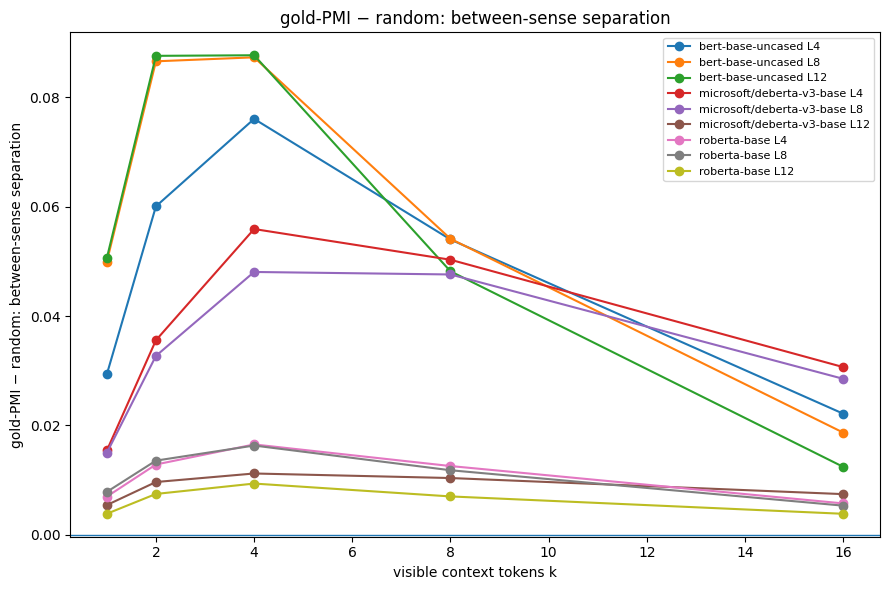
\includegraphics[width=\linewidth]{../figures/controlled_between_sense_separation.png}
\end{minipage}\hfill
\begin{minipage}{0.49\textwidth}
\centering
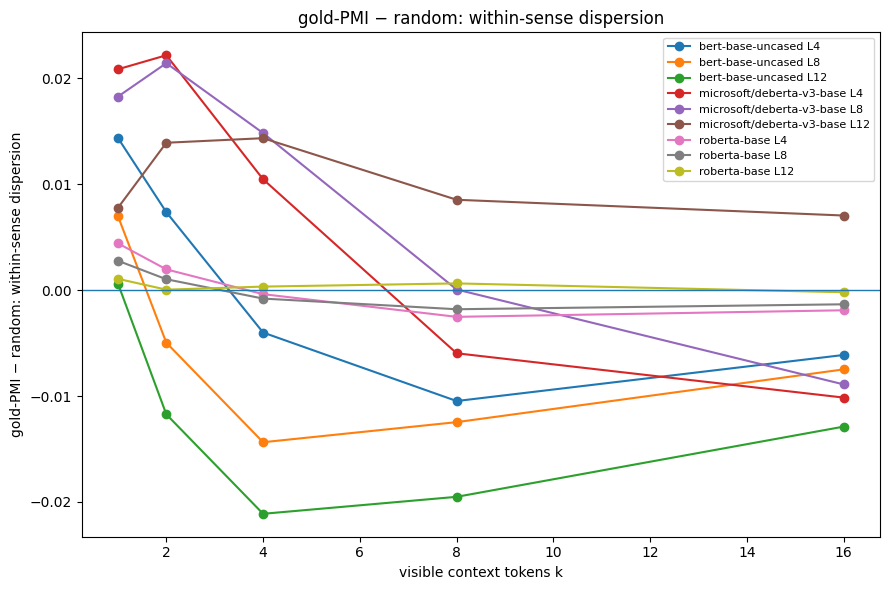
\includegraphics[width=\linewidth]{../figures/controlled_within_sense_dispersion.png}
\end{minipage}
\caption{Controlled diagnostic-minus-random effects. Between-sense separation is consistently positive, while within-sense dispersion has model-dependent trajectories. Raw magnitudes are interpreted only within model families.}
\label{fig:controlled}
\end{figure*}

The BERT deletion check preserves the qualitative between-sense direction, but equivalent artifact controls were not run for RoBERTa and DeBERTa-v3.

\subsection{A diagnostic cue changes more than a pure sense coordinate}
From an identical base context, a diagnostic cue increases linear sense accessibility relative to matched controls by a mean of \textbf{+0.265 nats}. The update also places a larger fraction of its energy in the supervised sense subspace (\textbf{+0.032} diagnostic-minus-control on average).

At the same time, structural similarity to the pre-cue state is lower under diagnostic cues: mean CKA diagnostic-minus-control is \textbf{-0.050}, and orthogonal residual variation is positive in most aggregate cells. The picture ``old vector + one sense-only displacement'' is therefore incomplete.

A fresh decoder fit after the update changes old-context reconstruction only slightly relative to control (\textbf{+0.00194} cosine on average), while a decoder trained on the base state transfers less well (\textbf{-0.00802}). Together with lower CKA, this is consistent with changed representational organization rather than indiscriminate loss of the fixed old-context target. It does not identify a unique transformation.

\begin{figure}[t]
\centering
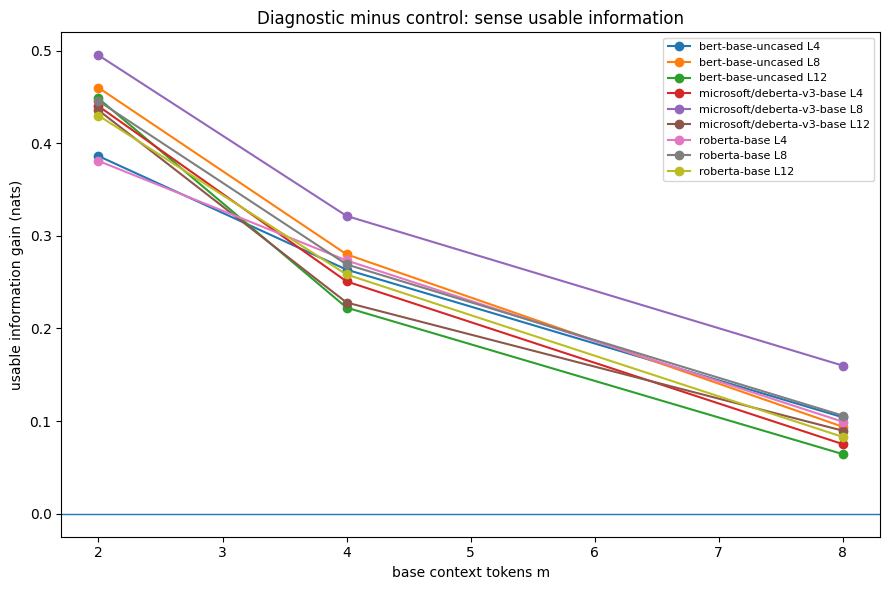
\includegraphics[width=\columnwidth]{../figures/nested_sense_accessibility.png}
\caption{Diagnostic-minus-control linear sense accessibility from the same pre-cue base context.}
\label{fig:nested}
\end{figure}

\subsection{Non-oracle context points in the same direction}
When context expands by distance alone, linear sense accessibility usually rises from 2 to 16 visible tokens. Mean usable-information gains are positive for every model/layer/transition in the executed notebook, with diminishing gains at richer contexts. The descriptive correlation between accessibility gain and supervised sense-update alignment is positive in all nine model/layer settings, strongest for BERT and weaker for DeBERTa-v3 layer 12. Because each word contributes multiple transitions, these are effect sizes rather than naive independent-point significance tests.

\subsection{Linear erasure leaves most of the fixed lexical target recoverable}
LEACE substantially reduces held-out linear sense accessibility. Table~\ref{tab:leace} shows absolute values averaged over base sizes. Across the tested model/layer settings, the corresponding old-context reconstruction loss is roughly 1.0--1.5\%.

\begin{table}[t]
\centering
\small
\begin{tabular}{lrrrr}
\toprule
Model & L & $I_V$ pre & $I_V$ post & Acc. post\\
\midrule
BERT & 8 & .587 & .183 & .586\\
BERT & 12 & .621 & .199 & .590\\
RoBERTa & 8 & .437 & .100 & .563\\
RoBERTa & 12 & .497 & .143 & .575\\
DeBERTa-v3 & 8 & .341 & -.005 & .550\\
DeBERTa-v3 & 12 & .076 & -.183 & .510\\
\bottomrule
\end{tabular}
\caption{Held-out linear sense accessibility before and after LEACE. Negative $I_V$ means the fitted probe is worse than the null predictor under this definition.}
\label{tab:leace}
\end{table}

This supports partial \emph{linear} separability between the removed sense signal and the fixed lexical context target. It does not imply nonlinear independence or complete concept deletion.

\subsection{External semantic alignment}
On RAW-C, target-token cosine similarity correlates positively with graded human relatedness in every model/layer setting (Spearman $\rho=.438$--$.693$). Same-versus-different-sense AUC ranges from .764 to .912. This is an external validity check for the representation geometry, not a replication of the intervention and not evidence that humans and models share a mechanism.

\section{What the result does and does not buy us}
The strongest conclusion is intentionally small: \textbf{more recoverable lexical-sense information does not require a universal collapse of same-sense representation geometry.} A contextual token can become easier to classify by coarse sense while still encoding distinctions among events, topics, entities, syntax, and discourse. Between-sense structure can sharpen while within-sense degrees of freedom remain.

The phrase \emph{sense-directed reorganization} summarizes four observations: controlled evidence differentiates senses; diagnostic updates contain a stronger supervised sense-related component; broader structural similarity changes; and a fixed old-context target is not proportionately destroyed. None of these observations establishes a universal transformer mechanism.

The main threats are concrete. The sense subspace and probe share supervision; a label-permutation or matched-random-subspace null would sharpen the ``sense-directed'' interpretation. The TF-IDF/SVD target is low-dimensional and lexical; richer independently defined context targets could reveal losses it misses. The masking artifact check is BERT-specific. The controlled dataset covers 19 English nouns with coarse senses. Finally, geometry itself is representation-dependent, so raw cross-model distances are not common units.

These limits narrow the claim, but they do not change the simplest observation: the same manipulation that makes senses easier to distinguish does not produce a common within-sense contraction trajectory across the three encoders.

\section{Conclusion}
A geometric intuition can be useful even when it fails. If contextual disambiguation were equivalent to a shrinking same-sense cloud, diagnostic evidence should reliably reduce within-sense dispersion. It does not. Across the tested encoders, the stable effect is increased differentiation between senses, accompanied by model-dependent within-sense geometry and broader changes under nested cue interventions. Context can therefore make lexical sense more accessible without making the representation geometrically simple.

\begin{thebibliography}{99}\small
\bibitem{belrose2023} N. Belrose et al. LEACE: Perfect linear concept erasure in closed form. \emph{NeurIPS}, 2023.
\bibitem{ethayarajh2019} K. Ethayarajh. How contextual are contextualized word representations? Comparing the geometry of BERT, ELMo, and GPT-2. \emph{EMNLP-IJCNLP}, 2019.
\bibitem{hewitt2019} J. Hewitt and P. Liang. Designing and interpreting probes with control tasks. \emph{EMNLP-IJCNLP}, 2019.
\bibitem{hu2026} Z. Hu, L. Niu, and S. Varma. Language Models Represent and Transform Concepts with Shared Geometry. arXiv:2607.04525, 2026.
\bibitem{loureiro2021} D. Loureiro et al. Analysis and evaluation of language models for word sense disambiguation. \emph{Computational Linguistics}, 47(2):387--443, 2021.
\bibitem{ma2025} M. K.-H. Ma, X. Chenwei, W. Wang, and W. S. Wang. Exploring Layer-wise Representations of English and Chinese Homonymy in Pre-trained Language Models. \emph{Findings of ACL}, 2025.
\bibitem{riviere2025} P. D. Rivi\`ere, A. L. Beatty-Mart\'inez, and S. Trott. Evaluating Contextualized Representations of (Spanish) Ambiguous Words: A New Lexical Resource and Empirical Analysis. \emph{NAACL}, 2025.
\bibitem{rivieretrott2025} P. D. Rivi\`ere and S. Trott. Start Making Sense(s): A Developmental Probe of Attention Specialization Using Lexical Ambiguity. arXiv:2511.21974, 2025.
\bibitem{scott2026} K. J. Scott, N. Pat, and V. Liesaputra. Divergent large language model predictions from convergent representations in ambiguous word pairs. arXiv:2608.01816, 2026.
\bibitem{timkey2021} W. Timkey and M. van Schijndel. All bark and no bite: Rogue dimensions in transformer language models obscure representational quality. \emph{EMNLP}, 2021.
\bibitem{trott2021} S. Trott and B. Bergen. RAW-C: Relatedness of Ambiguous Words in Context. \emph{ACL-IJCNLP}, 2021.
\bibitem{xiong2026} H.-D. Xiong et al. Large language models reorganize representational geometry during in-context learning. arXiv:2605.28854, 2026.
\end{thebibliography}

\end{document}
